\documentclass{article}
\usepackage{amsmath,amsfonts,amsthm,amssymb,chemfig,chemformula,fullpage,graphicx,multicol,multirow,parskip,setspace}

\onehalfspacing

\begin{document}
    \section*{VSEPR molecular geometry table}
    
    \begin{figure}[htb]
        \centering
        \includegraphics[width=6.5in]{figures/vsepr.jpg}
    \end{figure}
    \pagebreak

    \section*{Point group flowchart}
    
    \begin{figure}[htb]
        \centering
        \includegraphics[width=6.5in]{figures/flowchart.png}
    \end{figure}
    \pagebreak

    \section*{$C_{3v}$ Cayley table}
    
    \begin{table}[htb]
        \centering
        \renewcommand{\arraystretch}{1.5}
        \begin{tabular}{lcr}
            \begin{tabular}{l}
                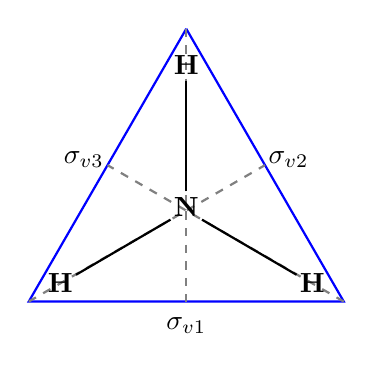
\begin{tikzpicture}[scale=2]
                    \coordinate (one) at (0,1.732);
                    \coordinate (two) at (1,0);
                    \coordinate (three) at (-1,0);
                    \coordinate (onetwo) at (0.5,0.866);
                    \coordinate (twothree) at (0,0);
                    \coordinate (onethree) at (-0.5,0.866);
                    \draw [blue,thick] (one)--(two)--(three)--(one);
                    \draw [gray,thick,dashed] (one)--(twothree);
                    \draw [gray,thick,dashed] (two)--(onethree);
                    \draw [gray,thick,dashed] (three)--(onetwo);
                    \draw [black,thick,solid] (0,0.7)--(0,1.4);
                    \draw [black,thick,solid] (-0.1,0.52)--(-0.7,0.17);
                    \draw [black,thick,solid] (0.1,0.52)--(0.7,0.17);
                    \node at (0,-0.15) {$\sigma_{v1}$};
                    \node at (0.65,0.9) {$\sigma_{v2}$};
                    \node at (-0.65,0.9)
                    {$\sigma_{v3}$};
                    \node at (0,0.6) {\textbf N};
                    \node at (0,1.5) {\textbf H};
                    \node at (-0.8,0.12) {\textbf H};
                    \node at (0.8,0.12) {\textbf H};
                \end{tikzpicture}\\
                \begin{tabular}{l}
                    $E$: Identity\\
                    $C_3$: $120^{\circ}$, counterclockwise\\
                    $C_3^2$: $240^{\circ}$, counterclockwise
                \end{tabular}
            \end{tabular}
            & \hspace{0.25in} &
            \begin{tabular}{cc|cccccc}
                & & \multicolumn{6}{c}{$g$}\\
                & $f \circ g$ & $E$ & $C_3$ & $C_3^2$ & $\sigma_{v1}$ & $\sigma_{v2}$ & $\sigma_{v3}$\\
                \hline
                \multirow{6}{*}{$f$} & $E$ & $E$ & $C_3$ & $C_3^2$ & $\sigma_{v1}$ & $\sigma_{v2}$ & $\sigma_{v3}$\\
                & $C_3$ & $C_3$ & $C_3^2$ & $E$ & $\sigma_{v3}$ & $\sigma_{v1}$ & $\sigma_{v2}$\\
                & $C_3^2$ & $C_3^2$ & $E$ & $C_3$ & $\sigma_{v2}$ & $\sigma_{v3}$ & $\sigma_{v1}$\\
                & $\sigma_{v1}$ & $\sigma_{v1}$ & $\sigma_{v2}$ & $\sigma_{v3}$ & $E$ & $C_3$ & $C_3^2$\\
                & $\sigma_{v2}$ & $\sigma_{v2}$ & $\sigma_{v3}$ & $\sigma_{v1}$ & $C_3^2$ & $E$ & $C_3$\\
                & $\sigma_{v3}$ & $\sigma_{v3}$ & $\sigma_{v1}$ & $\sigma_{v2}$ & $C_3$ & $C_3^2$ & $E$
            \end{tabular}
        \end{tabular}
    \end{table}

    \section*{$C_{2v}$ Cayley table}
    
    \begin{table}[ht]
        \centering
        \renewcommand{\arraystretch}{1.5}
        \begin{tabular}{lcr}
            \begin{tabular}{l}
                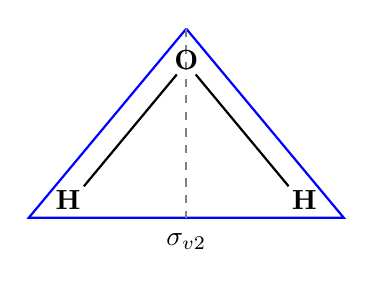
\begin{tikzpicture}[scale=2]
                    \coordinate (one) at (0,1.2);
                    \coordinate (two) at (1,0);
                    \coordinate (three) at (-1,0);
                    \coordinate (onetwo) at (0.5,0.866);
                    \coordinate (twothree) at (0,0);
                    \coordinate (onethree) at (-0.5,0.866);
                    \draw [blue,thick] (one)--(two)--(three)--(one);
                    \draw [gray,thick,dashed] (one)--(twothree);
                    \draw [black,thick,solid] (-0.06,0.91)--(-0.65,0.2);
                    \draw [black,thick,solid] (0.06,0.91)--(0.65,0.2);
                    \node at (0,-0.15) {$\sigma_{v2}$};
                    \node at (0,1) {\textbf O};
                    \node at (-0.75,0.11)
                    {\textbf H};
                    \node at (0.75,0.11)
                    {\textbf H};
                \end{tikzpicture}\\
                \begin{tabular}{l}
                    $E$: Identity\\
                    $C_2$: $180^{\circ}$\\
                    $\sigma_{v1}$: Reflection over molecular plane
                \end{tabular}
            \end{tabular}
            & \hspace{0.25in} &
            \begin{tabular}{cc|cccc}
                & & \multicolumn{4}{c}{$g$}\\
                & $f \circ g$ & $E$ & $C_2$ & $\sigma_{v1}$ & $\sigma_{v2}$\\
                \hline
                \multirow{4}{*}{$f$} & $E$ & $E$ & $C_2$ & $\sigma_{v1}$ & $\sigma_{v2}$\\
                & $C_2$ & $C_2$ & $E$ & $\sigma_{v2}$ & $\sigma_{v1}$\\
                & $\sigma_{v1}$ & $\sigma_{v1}$ & $\sigma_{v2}$ & $E$ & $C_2$\\
                & $\sigma_{v2}$ & $\sigma_{v2}$ & $\sigma_{v1}$ & $C_2$ & $E$
            \end{tabular}
        \end{tabular}
    \end{table}

    \section*{Coordinate axes used for \ch{H2O} and \ch{NH3}}
    \begin{center}\includegraphics[width=1.5in]{axes/waterxyz.png} \includegraphics[width=2in]{axes/ammoniaxyz.png}\end{center}
    \pagebreak

    \section*{Properties of character tables}

    Let $\chi_i(C)$ represent the character of class $C$ in the $i$th irrep.
    
    \begin{itemize}
        \item The number of symmetry operations is the order of the group, $h$.
        \item If symmetry operations are grouped by conjugacy class $C$, we show how many operations are in the class, $n_C$, in the top row. For example, if there are three rotations in the $C_2$ class, the top row will be labeled $3C_2$. We will call $n_C$ the multiplicity of the class.
        \item The number of irreps equals the number of classes. That is, the character table needs to have the same number of rows and columns.
        \item Taking the sum over all of the irreps, we have \[\sum_i\chi_i^2(E)=h,\] where $E$ is the identity operation.
        \item For the $i$th irrep, we have \begin{equation}\sum_C n_C \chi_i^2(C)=h,\label{sumsq}\end{equation} where the sum is taken over all of the conjugacy classes.
        \item \textbf{Orthogonality Theorem.} Irreps are orthogonal. We have, for the $i$th and $j$th irreps, \begin{equation}
        \sum_C n_C \chi_i(C)\chi_j(C)=h\delta_{ij},\label{orthog}\end{equation} where $\delta_{ij}$ is the Kronecker delta. This form of the orthogonality formula is easily proven from the fact that every symmetry operation in a given conjugacy class has the same character. When $i=j$, \eqref{orthog} reduces to \eqref{sumsq}, and when $i\neq j$, we have \[\sum_C n_C \chi_i(C)\chi_j(C)=0.\] 
        \item One irrep has characters that are all $1$, which is labeled $A_1$.
        \item Each irrep must be distinct.
    \end{itemize}
    \pagebreak

    \section*{$C_{2v}$ character table}
    
    \begin{table}[h]
        \centering
        \renewcommand{\arraystretch}{1.5}
        \begin{tabular}{c|cccc|c|c}
            $C_{2v}$ & $E$ & $C_2$ & $\sigma_{v1}~(xz)$ & $\sigma_{v2}~(yz)$ & &\\
            \hline
            $A_1$ & 1 & 1 & 1 & 1 & $z$ & $x^2, y^2, z^2$\\
            $A_2$ & 1 & 1 & -1 & -1 & $R_z$ & $xy$\\
            $B_1$ & 1 & -1 & 1 & -1 & $x, R_y$ & $xz$\\
            $B_2$ & 1 & -1 & -1 & 1 & $y, R_x$ & $yz$\\
        \end{tabular}
    \end{table}

    \section*{$C_{3v}$ character table}
    
    \begin{table}[h]
        \centering
        \renewcommand{\arraystretch}{1.5}
        \begin{tabular}{c|ccc|c|c}
            $C_{3v}$ & $E$ & $2C_3$ & $3\sigma_{v}$ & &\\
            \hline
            $A_1$ & 1 & 1 & 1 & $z$ & $x^2+y^2, z^2$\\
            $A_2$ & 1 & 1 & -1 & $R_z$ &\\
            $E$ & 2 & -1 & 0 & $(x,y), (R_x,R_y)$ & $(x^2-y^2,xy),(xz,yz)$\\
        \end{tabular}
    \end{table}

    \section*{Expressing reducible representations in terms of irreps}
    
    The reducible representation $\Gamma$ can be written as a linear combination of the irreducible representations (irreps). That is, for each class $C$, and for each character $\chi(C)$ in $\Gamma$, with corresponding character $\chi_i(C)$ in the $i$th irrep, there exist coefficients $n_1, n_2,\ldots$ such that \begin{equation}\chi_C=\sum_in_i\chi_i(C).\label{lincomb}\end{equation}
    
    \textbf{Lemma 1.} Each coefficient $n_i$ in \eqref{lincomb} is given by
    \[n_i=\frac1h\sum_Cn_C\chi(C)\chi_i(C),\]
    where $h$ is the order of the group.

    \section*{Molecular vibration demo}

    \begin{verbatim}https://www.chem.purdue.edu/jmol/vibs/h2o.html\end{verbatim}
    \pagebreak

    \section*{IR spectrum of water}
    
    \begin{figure}[hbp]
        \centering
        \includegraphics[width=6in]{figures/irwater.png}
    \end{figure}

    \section*{Chirality and optical activity}

    \begin{center}\includegraphics[width=3in]{figures/enantiomers.png}\end{center}

    \begin{figure}[htbp]
        \centering
        \includegraphics[width=5in]{figures/chiral.jpg}
    \end{figure}
\end{document}